\documentclass{article}
\usepackage{graphicx} % Required for inserting images
\usepackage{listings}

\title{CSE222A HW7}
\author{Caden Roberts}
\date{March 14 2025}

\begin{document}

\maketitle
\begin{flushleft}
\section{Design Setup and Baseline PPA}
\subsection{\bf{config.yaml}}
\noindent\makebox[\linewidth]{\rule{\paperwidth}{0.4pt}}
\begin{lstlisting}
MACROS: 
  sky130_sram_1kbyte_1rw1r_32x256_8:
    gds: dir::src/mem/sky130_sram_1kbyte_1rw1r_32x256_8.gds
    lef: dir::src/mem/sky130_sram_1kbyte_1rw1r_32x256_8.lef 
    lib: 
      "*": dir::src/mem/sky130_sram_1kbyte_1rw1r_32x256_8_TT_1p8V_25C.lib
\end{lstlisting}
\bf{\begin{lstlisting}
    instances:
      mem_inst0:
        orientation: N
        location: [300, 800]
      mem_inst1:
        orientation: N
        location: [950, 800]

RUN_HEURISTIC_DIODE_INSERTION: true # change from false to true
GRT_RESIZER_SETUP_SLACK_MARGIN: 0.8 # increase to 0.8ns from 0.025ns
GRT_RESIZER_HOLD_SLACK_MARGIN: 0.8 # increase to 0.8ns from 0.05ns
GRT_RESIZER_HOLD_MAX_BUFFER_PCT: 60 # increase to 60% from 50%
GRT_RESIZER_SETUP_MAX_BUFFER_PCT: 100 # increase to 100% from 50%
PL_RESIZER_HOLD_MAX_BUFFER_PCT: 45 # decrease from 50% to 45%
PL_RESIZER_HOLD_SLACK_MARGIN: 0.6 # increase from 0.1ns to 0.6ns
RUN_POST_GRT_RESIZER_TIMING: true # change to true from false
DIODE_ON_PORTS: 'both'  # change to both from none
GRT_ANTENNA_ITERS: 30 # change to 30 from 3
GRT_ANTENNA_MARGIN: 75} # change to 75% from 10%
\end{lstlisting}}
\noindent\makebox[\linewidth]{\rule{\paperwidth}{0.4pt}}
{\large I changed no other parameters from the example.yaml; what is highlighted are variables I changed to achieve my Baseline PPA, pass DRC, LVS, and remove all setup and hold violations. I created the instances as instructed in office hours, otherwise, we get expected errors.
Below is how I used each variable:}
\begin{itemize}
\item \bf{RUN\_HEURISTIC\_DIODE\_INSERTION:}
\\Definition: Enables the Odb.HeuristicDiodeInsertion step.
\\Explanation: Enabling this step greatly reduced antenna errors and allowed me to pass the antenna stage without errors.
\item \bf{GRT\_RESIZER\_SETUP\_SLACK\_MARGIN:}
\\Definiton: Specifies a time margin for the slack when fixing setup violations.
\\Explanation: By increasing the setup slack margin to 0.8ns from 0.025ns the global resizer has more room to optimize the timing paths and avoid setup violations.
\item \bf{GRT\_RESIZER\_HOLD\_SLACK\_MARGIN:}
\\Definition: Specifies a time margin for the slack when fixing hold violations. Normally the resizer will stop when it reaches zero slack. This option allows you to overfix.
\\Explanation: Raising the hold slack margin to 0.8ns from 0.05ns allows more optimization for adjustments in the hold paths. We could fix the hold paths past zero-slack so that data doesn't arrive too fast. This eliminates hold violations.
\item \bf{GRT\_RESIZER\_HOLD\_MAX\_BUFFER\_PCT:}
\\Definition: Specifies a max number of buffers to insert to fix hold violations. This number is calculated as a percentage of the number of instances in the design.
\\Explanation: Allowing for 60 instead of 50 percent of the design instances to be buffered for hold fixes ensures enough buffers will be added to delay signals appropriately, resolving hold issues.
\item \bf{GRT\_RESIZER\_SETUP\_MAX\_BUFFER\_PCT:}
\\Definition: Specifies a max number of buffers to insert to fix setup violations. This number is calculated as a percentage of the number of instances in the design.
\\Explanation: Raising the max allowable buffer percentage for setup fixes to 100 percent from 50 enables aggressive buffer insertion. This is crucial for addressing setup violations by delaying signals to meet timing requirements.
\item \bf{PL\_RESIZER\_HOLD\_MAX\_BUFFER\_PCT:}
\\Definition: Specifies a max number of buffers to insert to fix hold violations. This number is calculated as a percentage of the number of instances in the design.
\\Explanation: Restricting the maximum buffer insertion to 45 percent from 50 helps prevent worsening slew performance from over-buffering during placement. This change is minor to still provide enough correction to remove hold violations.
\item \bf{PL\_RESIZER\_HOLD\_SLACK\_MARGIN:}
\\Definition: Specifies a time margin for the slack when fixing hold violations. Normally the resizer will stop when it reaches zero slack. This option allows you to overfix.
\\Explanation: Increasing the hold slack margin during placement to 0.6ns from 0.1ns gives the placement optimizer room to fix hold issues. A larger margin ensures adjustments made do not create new timing violations or worsen slew.
\item \bf{RUN\_POST\_GRT\_RESIZER\_TIMING:}
\\Definiton: Enables resizer timing optimizations after clock tree synthesis using the OpenROAD.ResizerTimingPostCTS step.
\\Explanation: Enabling this is essential for variables like
\\GRT\_RESIZER\_HOLD\_SLACK\_MARGIN to be effective.
\item \bf{DIODE\_ON\_PORTS:}
\\Definition: Always insert diodes on ports with the specified polarities.
\\Explanation: 'both' allows RUN\_HEURISTIC\_DIODE\_INSERTION to insert diodes on input and output ports, helping with antenna errors.
\item \bf{GRT\_ANTENNA\_ITERS:}
\\Definition: The maximum number of iterations for global antenna repairs.
\\Explanation: Increasing the iterations for global antenna repair from 3 to 30 helps ensure correction of antenna issues. 
\item \bf{GRT\_ANTENNA\_MARGIN:}
\\Definition: The margin to over fix antenna violations.
\\Explanation: Expanding the antenna margin to 75 percent from 10 percent helps ensure antenna repairs don't greatly affect timing.
\end{itemize}
\noindent\makebox[\linewidth]{\rule{\paperwidth}{0.4pt}}
\subsection{pin\_order.cfg}
\begin{lstlisting}
#N
@min_distance=0.5
alert_.*
core_sleep_o

#S
rst_ni
test_en_i
fetch_enable_i
debug_req_i

#E
clk_i
irq_.*
hart_id_i\[.*\]
boot_addr_i\[.*\]

#W
instr_.*
data_.*
\end{lstlisting}
\noindent\makebox[\linewidth]{\rule{\paperwidth}{0.4pt}}
{\large Below is what my pin\_order.cfg is doing:}
\begin{itemize}
\item \#N Sets min distance to 0.5 microns. Places core\_sleep\_o and any pins starting with alert\_ on the North side.
\item \#S Places rst\_ni, test\_en\_i, fetch\_enable\_i and debug\_req\_i on the South side.
\item \#E Places clk\_i, any pin starting with irq\_, any pin index-able at hard\_id\_i[ ] and any pin index-able at boot\_addr\_i[ ] on the East side.
\item \#W Places any pin starting with instr\_ or data\_ on the west side.
\end{itemize}
\noindent\makebox[\linewidth]{\rule{\paperwidth}{0.4pt}}
\subsection{base.sdc}
\begin{lstlisting}
1  current_design top
2  set ::env(IO_SYNC) 0
3  set clock_port clk_i
4  set clock_period 100
5  create_clock -name $clock_port -period $::env(CLOCK_PERIOD)
[get_ports $clock_port]
6  set clk_input [get_port $clock_port]
7  set clk_indx [lsearch [all_inputs] $clk_input]
8  set all_inputs_wo_clk [lreplace [all_inputs] $clk_indx
$clk_indx ""]
9  set_input_delay 2 -clock $clock_port $all_inputs_wo_clk
10 set_output_delay 2 -clock $clock_port [all_outputs]
11 set_driving_cell -lib_cell sky130_fd_sc_hd__dfxtp_1 -pin
{Q} $all_inputs_wo_clk
12 set_clock_uncertainty 0.1 [get_clocks $clock_port]
13 set_input_transition 0.05 $all_inputs_wo_clk
14 set_load 0.006 [all_outputs]
\end{lstlisting}
\noindent\makebox[\linewidth]{\rule{\paperwidth}{0.4pt}}
{\large Below is how each line met assignment requirements:}
\begin{enumerate}
\item Sets the active design to top.
\item Disables automatic I/O port synchronization adjustments.
\item Define clock\_port as the port clock\_i.
\item Define clock\_period as 100ns.
\item Creates a clock constraint using the [get\_ports \$clock\_port] port. The clock is named after the value in \$clock\_port (clk\_i) and its period is set to CLOCK\_PERIOD.
\item Define clk\_input as the port at [get\_port \$clock\_port]
\item Searches the list [all\_inputs] to find the index of \$clk\_input and sets clk\_indx to it.
\item Uses lreplace to remove the clock\_port from the [all\_inputs] list. The resulting list is stored in all\_inputs\_wo\_clk (contains all inputs without the clock).
\item Sets all inputs (\$all\_inputs\_wo\_clk) to have an input delay of 2ns relative to the clock edge on \$clock\_port.
\item Sets all outputs ([all\_outputs]) to have an output delay of 2ns relative to the clock edge on \$clock\_port. 
\item Sets driving cell characteristics. The delay and transition are to be modeled using the cell sky130\_fd\_sc\_hd\_\_dfxtp\_1 at pin Q.
\item Adds a clock uncertainty of 0.1ns to the clock [get\_clocks \$clock\_port]. 
\item Adds an input slew of 0.05ns to \$all\_inputs\_wo\_clk.
\item Sets a load capacitance of 0.006pF on [all\_outputs].
\end{enumerate}
\noindent\makebox[\linewidth]{\rule{\paperwidth}{0.4pt}}
\subsection{signoff.sdc}
\begin{lstlisting}
source base.sdc
set_propagated_clock [get_clocks $clock_port]
\end{lstlisting}
\noindent\makebox[\linewidth]{\rule{\paperwidth}{0.4pt}}
{\large For signoff.sdc, I source base and propagate the clock.}
\noindent\makebox[\linewidth]{\rule{\paperwidth}{1.2pt}}
\section{What are your final improved PPA metrics?}
Here are the Power, Performance, and Area metrics:
\begin{lstlisting}
{
    ...
    "power__internal__total": 0.010155528783798218,
    "power__switching__total": 0.01924416422843933,
    "power__leakage__total": 3.847679909085855e-05,
    "power__total": 0.029438169673085213,
    ...
    "clock__skew__worst_hold": 7.287969545249306,
    "clock__skew__worst_setup": 2.6642533378023514,
    "timing__hold__ws": 0.03751354888461996,
    "timing__setup__ws": 39.81512121581859,
    "timing__hold_r2r__ws": 0.705701,
    "timing__setup_r2r__ws": 39.815121,
    ...
    "design__die__area": 2715200,
    "design__core__area": 2657620,
    ...
}
\end{lstlisting}
Power: Total power is 0.029438169673085213 W. \\ Performance: Worst skew hold is 7.29ns and worst skew setup is 2.66ns. Worst hold is 0.038ns and worst setup is 39.82ns. \\ Area: Die area is 2715200 microns squared and core area is 2657620 microns squared.
\section{Describe the Power breakdown. How much power do the sequential and combinational gates
take in your design?}
Here are cell counts:
\begin{lstlisting}
{
    ...
    "design__instance__count__class:macro": 2,
    "design__instance__count__class:buffer": 30,
    "design__instance__count__class:inverter": 191,
    "design__instance__count__class:sequential_cell": 1932,
    "design__instance__count__class:multi_input_combinational_cell":
    10110,
    ...
}
\end{lstlisting}
Combinational =  10110/(10110+1932+191+30+2) * 0.029438169673085213 = 0.02426578845 W or 82.43\% of total power.\\
Sequential = 1932/(10110+1932+191+30+2) * 0.029438169673085213 = 0.00463714176 W or 15.75\% of total power.
\section{What is your critical path and why is it critical? For example: How many stages is it? Does it have long wires (show an image of it)? Does it have high fanout?}
I assume my critical path is along the max\_ss\_100C\_1v60 corner or min\_ff\_n40C\_1v95 corner as they have the worst hold and setup skew respectively. Unfortunately, I ran into an error while trying to load the top.sdc and couldn't analyze timing paths:
\begin{lstlisting}
>>> read_sdc sdc/top.sdc
[ERROR STA-0453] 'sky130_fd_sc_hd__dfxtp_1' not found.
[ERROR GUI-0070] Error: top.sdc, 383 STA-0453
\end{lstlisting}

\section{What is your maximum clock skew? How much clock skew is on your critical path?}
Clock skews:
\begin{lstlisting}
{
    ...
    "clock__skew__worst_hold": 7.287969545249306,
    "clock__skew__worst_setup": 2.6642533378023514,
    "clock__skew__worst_hold__corner:max_ss_100C_1v60":
    7.287969545249306,
    "clock__skew__worst_setup__corner:min_ff_n40C_1v95":
    2.6642533378023514,
    ...
}
\end{lstlisting}
The worst hold skew is 7.29ns at the max\_ss\_100C\_1v60 corner and the worst setup skew is 2.66ns at the min\_ff\_n40C\_1v95 corner.
\section{How big is your design floorplan? What is your utilization?}
Floorplan and utilization:
\begin{lstlisting}
{
    ...
    "design__die__bbox": "0.0 0.0 1642.435 1653.155",
    "design__core__bbox": "5.52 10.88 1636.68 1640.16",
    "design__die__area": 2715200,
    "design__core__area": 2657620,
    "design__instance__utilization": 0.264001,
    ...
}
\end{lstlisting}
Die and core dimensions of "0.0 0.0 1642.435 1653.155" and "5.52 10.88 1636.68 1640.16" microns respectively. \\ Die area is 2715200 microns squared and core area is 2657620 microns squared. \\ Instance utilization is 26.4\%.
\section{What is the wirelength of your placement?}
Wirelength:
\begin{lstlisting}
{
    ...
    "route__wirelength": 1278545,
    ...
}
\end{lstlisting}
Route length is 1278545 microns.
\section{Where is the maximum congestion in your design? Physically show this in the GUI.}
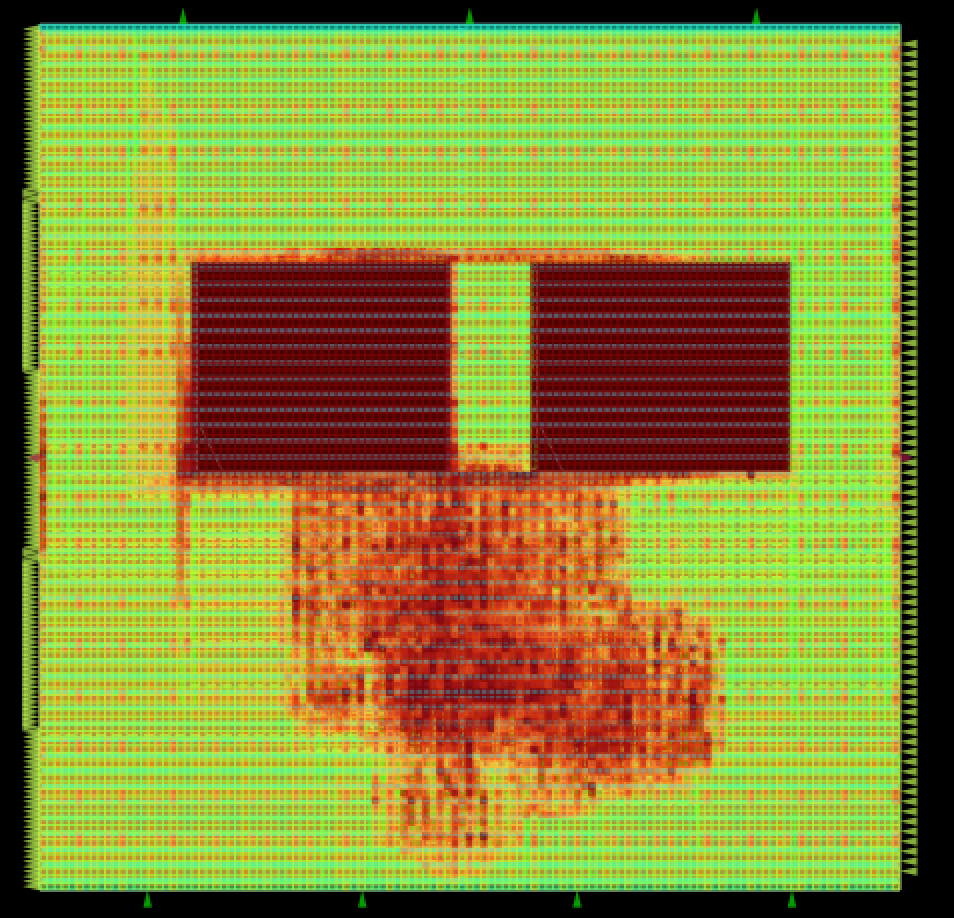
\includegraphics[width=10cm]{congestion.png} \\
Max congestion is seen in the 2 very dark red squares. There is little congestion surrounding them.
\section{Write a narrative of your approach to improve PPA. What did each option intend to improve and what were the results?}
I intended to improve PPA using DESIGN\_REPAIR\_MAX\_SLEW\_PCT, DESIGN\_REPAIR\_MAX\_CAP\_PCT, DIE\_AREA, CORE\_AREA, and clock speed. This would improve performance from the faster clock speed. Setting die and core area will reduce area. Power will improve from a better slew and capacitance. Beyond the improvements I didn't get to, the variables I configured above helped improve my PPA as well.

\section{Did improving one metric hurt another?}
Enhancing performance by reducing delay can hurt power efficiency if we insert buffers or increase drive strength. Enhancing performance with pipelining or extra logic can increase area. The converse is also true, where reducing area or increasing power efficiency can hurt performance.

\end{flushleft}
\end{document}
